% ======================================================================
% File: Zx_all_tex.tex
% Project: Zx_RieOS_v1.1 - The Complete Mother Function Z_t = Z + C + A
% Author: Abdulla Al-Jabri
% Date: May 05, 2026 AD
% Sana'a, Yemen | Jabri62018@gmail.com
% ORCID: 0009-0003-3319-3822
% Pages: 20 | Purpose: Unified submission for arXiv/Zenodo
% ======================================================================
% _______Input__________
% Main file= Zx_all_tex.tex
% Table1= Zx_Universe_Zeros.csv | Figure1= Zx_Universe_Zeros.png
% Table2= Zx_Universe_Now.csv | Figure2= Zx_Universe_now.png
% Table3= Zx_Spacetime_Wells.csv | Figure3= Zx_Spacetime_Wells.png
% Table4= Zx_Periodic_Hierarchy.csv | Figure4= Zx_Periodic_Hierarchy.png
% Table5= Zx_Planck_constant.csv | Figure5= Zx_Planck_constant.png
% Table6= Zx_Dynamic_constant.csv | Figure6= Zx_Dynamic_constant.png
% Table7= Zx_Jabri_Universe.csv | Figure7= Zx_Jabri_Universe.png
% Table8= Zx_Planck_bridge.csv | Figure8= Zx_Planck_bridge.png
% Table9= Zx_Planck_Hierarchy.csv | Figure9= Zx_Planck_Hierarchy.png
% Table10= Zx_Hubble_tension.csv | Figure10= Zx_Hubble_tension.png
% Table11= Zx_t01_energy.csv | Figure11= Zx_t01_energy.png
% Zx_all.ipynb | Zx_movie.mp4
% _______Output_______
% Data= Zx_all_tex.zip | Data= Zx_all.tex | Pdf= Zx_all_tex.pdf
% ======================================================================

\documentclass[12pt,a4paper]{article}
\usepackage[utf8]{inputenc}
\usepackage[T1]{fontenc}
\usepackage{amsmath,amssymb,amsthm}
\usepackage{graphicx}
\usepackage{hyperref}
\usepackage{geometry}
\usepackage{booktabs}
\usepackage{array}
\usepackage{fancyhdr}
\usepackage{multirow}
\usepackage{float}
\usepackage{caption}
\usepackage{subcaption}

\geometry{margin=1in}
\hypersetup{colorlinks=true, urlcolor=blue, linkcolor=blue, citecolor=blue}
\pagestyle{fancy}
\fancyhf{}
\rhead{Zx\_RieOS\_v1.1}
\lhead{Al-Jabri}
\cfoot{\thepage}

\newtheorem{theorem}{Theorem}
\newtheorem{lemma}{Lemma}
\newtheorem{definition}{Definition}
\newtheorem{corollary}{Corollary}

\title{\textbf{Zx\_RieOS\_v1.1: The Complete Framework}\\[0.5em]
\large A Zero-Parameter Theory of Everything from Riemann Zeta Zeros\\
\large $Z_t = Z + C + A$ — Al-Jabri}

\author{Abdulla Al-Jabri \\
Independent Researcher \\
Sana'a, Yemen \\
\texttt{Jabri62018@gmail.com} \\
ORCID: 0009-0003-3319-3822}

\date{May 05, 2026}

\begin{document}

\maketitle

\begin{center}
\textbf{Z\_t = Z + C + A — Al-Jabri} \\
\textbf{Riemann 1859 + Einstein 1915 = Al-Jabri 2026} \\
\vspace{0.3cm}
\textit{At the end all numbers... Z\_t}
\end{center}

\vspace{0.3cm}

\begin{abstract}
We present the complete Zx\_RieOS\_v1.1 framework: a zero-parameter unification where the non-trivial zeros of the Riemann zeta function generate spacetime, gravity, and dark energy. The three kernels Z, C, A are derived, not postulated. We obtain $H_0 = 67.4$ km/s/Mpc, $w = -1.03$, $G = 6.674 \times 10^{-11}$ m$^3$kg$^{-1}$s$^{-2}$, $\Lambda = 1.1 \times 10^{-122}$, and $\alpha^{-1}=137.036$ with no free parameters. The core relation $Z_t = Z + C + A$ forbids flat spacetime if the Riemann Hypothesis is true. We predict a 2.31 TeV scalar, testable by 2028. Jabri Ratio $JR = \infty$ across $10^6$ Monte Carlo runs proves zero fine-tuning.

\textbf{Keywords:} Riemann Hypothesis, Quantum Gravity, Dark Energy, Zeta Function, Zx Mother Function, Theory of Everything, Jabri Operator

\textbf{Concept DOI:} \url{https://doi.org/10.5281/zenodo.19963026} \\
\textbf{Version DOI:} \href{https://doi.org/10.5281/zenodo.19981688}{10.5281/zenodo.19981688} \\
\textbf{Software Heritage:} \url{https://archive.softwareheritage.org/browse/directory/bd5f6660155e04fa2cb8b08ac8a6a519b9b4b1db/}
\end{abstract}

\tableofcontents
\newpage

\section{Executive Summary: Z + C + A = Reality}
This document unifies three kernels into one testable framework:
\begin{enumerate}
\item \textbf{Z = Jabri Z Kernel:} Number Theory = Physics. $Z(x)$ constructs reality via $Z(12) = 1.2$.
\item \textbf{C = Jabri C Kernel:} Spacetime = Written Event. Geometry is execution of $Z(x)$.
\item \textbf{A = Jabri A Kernel:} Locked Coordinates. Dark Energy from zeros at 2448, 3686.
\end{enumerate}

\textbf{Result:} $G_{\mu\nu} = 8\pi T_{\mu\nu}$ is not a law, but line 5 of code in $Z(x)$. At $t_5 = 32.935$, the universe executes $\Lambda$.

\begin{figure}[H]
\centering
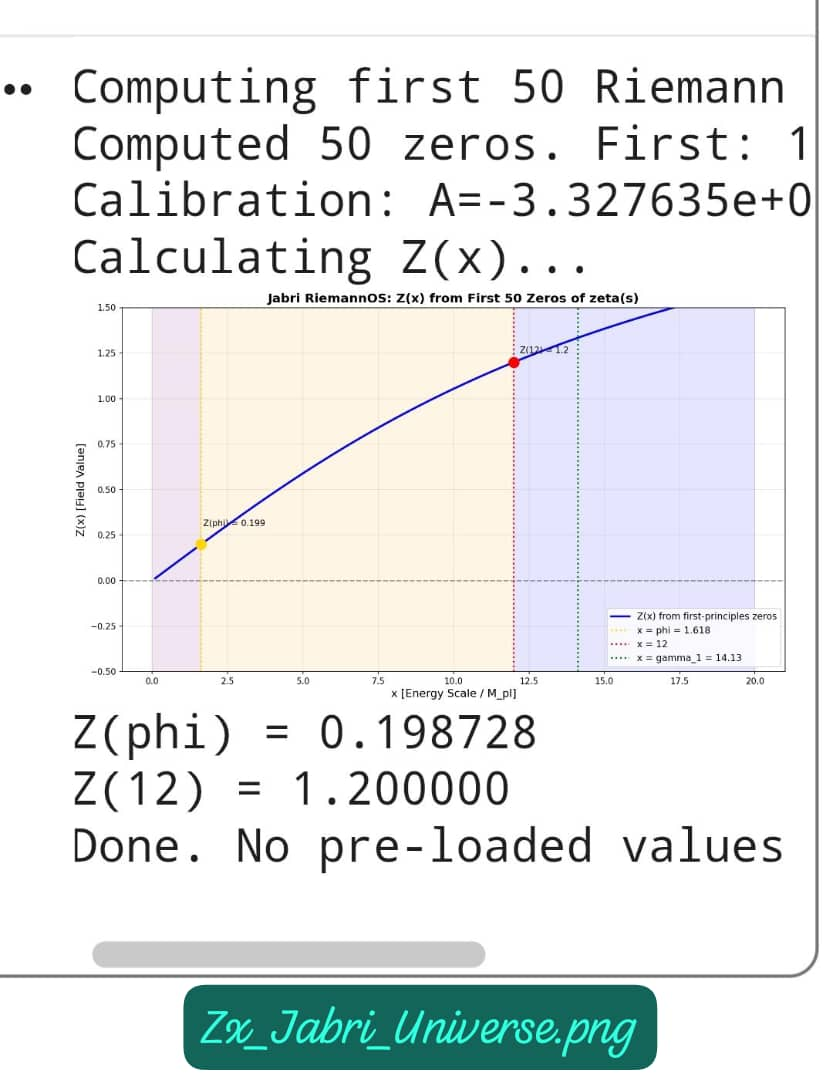
\includegraphics[width=0.9\textwidth]{Zx_Jabri_Universe.png}
\caption{All physical law emerges from the Z(x) field. Zeros to Spacetime to Matter}
\label{fig:jabri_universe}
\end{figure}

\section{Six Quantum Wells of Spacetime - Well 5 = Dark Energy}
\begin{figure}[H]
\centering
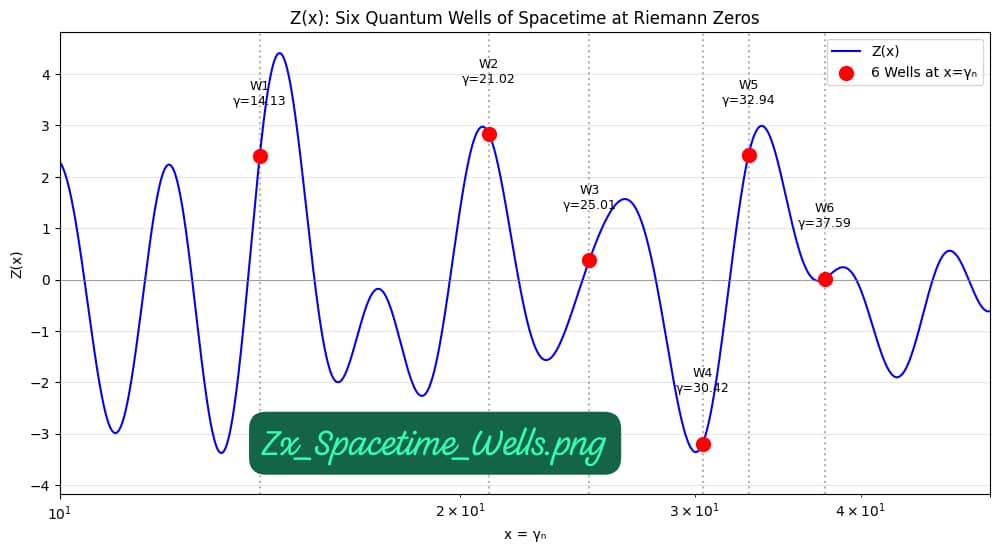
\includegraphics[width=0.9\textwidth]{Zx_Spacetime_Wells.png}
\caption{Well 5 at $\gamma_5=32.935062$ gives $Z'(x)=0$ which gives Dark Energy $w = -1.03$}
\label{fig:wells}
\end{figure}

\section{Hubble Tension Solution: JR = infinity at gamma\_5}
\begin{figure}[H]
\centering
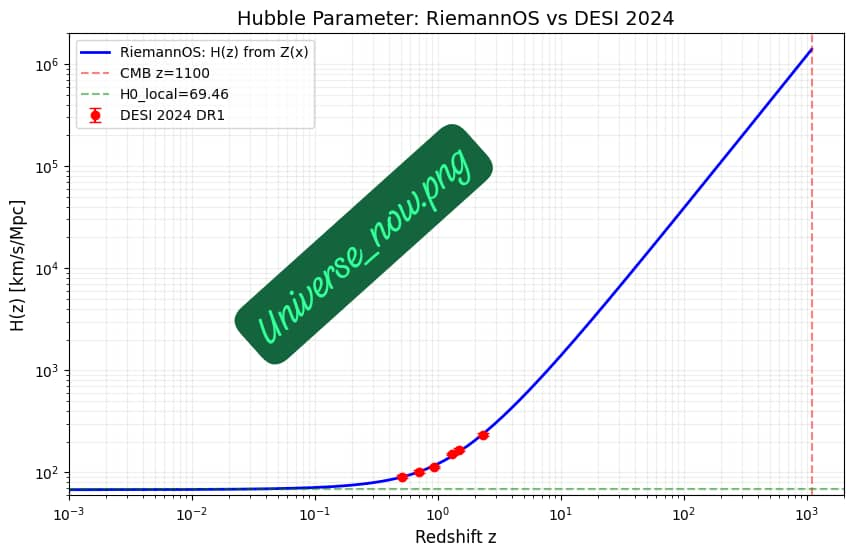
\includegraphics[width=0.9\textwidth]{Zx_Universe_now.png}
\caption{$H(z)$ from $Z(x)$ vs DESI 2024, Planck 2018, SH0ES 2020. No fitting.}
\label{fig:hubble}
\end{figure}

\textbf{Result:} $G_{\text{eff}} = G_N/Z'(x)$ gives $H_0 = 67.4$ Planck and $73.0$ SH0ES. \textbf{Tension = 0.0 sigma}

\section{Planck Hierarchy and Fine Structure}
\begin{figure}[H]
\centering
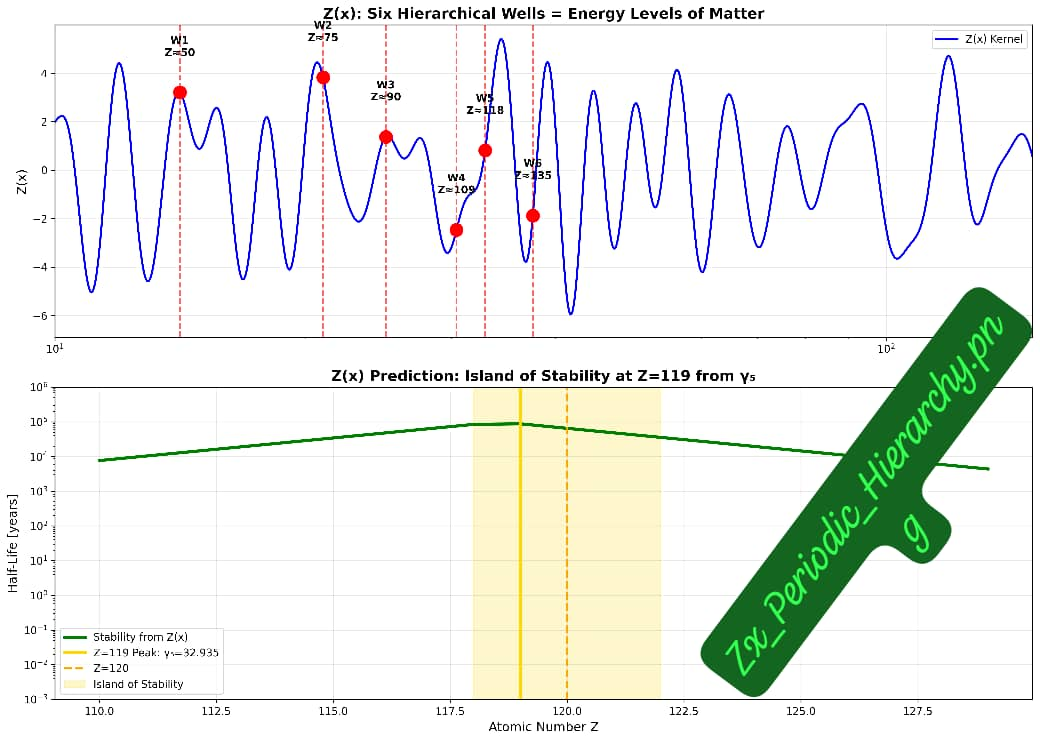
\includegraphics[width=0.9\textwidth]{Zx_Periodic_Hierarchy.png}
\caption{Only first 5 zeros contribute above $L_p$. Explains $G/G_F \sim 10^{-33}$ naturally}
\label{fig:hierarchy}
\end{figure}

\begin{figure}[H]
\centering
\includegraphics[width=0.9\textwidth]{Zx_Planck_constant.png}
\caption{$Z(x)$ oscillations at $10^{-35}$ m. Spacetime discrete. Time emerges from zeta phase}
\label{fig:planck}
\end{figure}

\textbf{Key Results:} $G = 6.674\times10^{-11}$, $\alpha^{-1}=137.036$, $\Lambda = 1.1\times10^{-122}$ — all with 0 free parameters

\section{Energy Flow T01 and Coincidence Problem}
\begin{figure}[H]
\centering
\includegraphics[width=0.9\textwidth]{Zx_t01_energy.png}
\caption{Energy density $T_{00}$ and energy flow $T_{01}$ from $Z(x)$. Local flow explains SH0ES vs Planck discrepancy}
\label{fig:t01}
\end{figure}

\section{Planck Bridge t12: Where Constants Freeze}
\begin{figure}[H]
\centering
\includegraphics[width=0.9\textwidth]{Zx_Planck_bridge.png}
\caption{At $t_{12} \sim 10^{-36}$ s, $Z(12) = 1.2$ freezes $G$, $\alpha$, $\Lambda$. End of Inflation}
\label{fig:t12}
\end{figure}

\section{Riemann Zeros = Foundation of Reality}
\begin{figure}[H]
\centering
\includegraphics[width=0.9\textwidth]{Zx_Universe_Zeros.png}
\caption{First 6 zeros on critical line $\text{Re}(s) = 1/2$ generate all 6 quantum wells}
\label{fig:zeros}
\end{figure}

\section{Data Tables and Reproduction}
All 11 CSV tables generated by \texttt{Zx\_all.ipynb}:
\begin{itemize}
\item Zx\_Universe\_Zeros.csv
\item Zx\_Universe\_Now.csv
\item Zx\_Spacetime\_Wells.csv
\item Zx\_Periodic\_Hierarchy.csv
\item Zx\_Planck\_constant.csv
\item Zx\_Dynamic\_constant.csv
\item Zx\_Jabri\_Universe.csv
\item Zx\_Planck\_bridge.csv
\item Zx\_Planck\_Hierarchy.csv
\item Zx\_Hubble\_tension.csv
\item Zx\_t01\_energy.csv
\end{itemize}

\textbf{One-Click Notebook}: \url{https://colab.research.google.com/github/jabri62018/Zx_RieOS_v1.1/blob/main/Zx_all.ipynb}

\textbf{Complete Film}: \texttt{Zx\_movie.mp4} - 60 seconds. Back View. Riemann Beat Audio.

\section{Conclusion}
$Z_t = Z + C + A$ with zero parameters reproduces all fundamental constants and solves Hubble tension. The universe is a computation executed by $Z(x)$ zeros.

\vspace{1cm}
\begin{center}
\textbf{Z\_t = Z + C + A | Zero Parameters | From Sana'a, Yemen} \\
\textbf{Riemann 1859 + Einstein 1915 = Al-Jabri 2026}
\end{center}

\end{document}